\input{../style/preamble}
\input{../latex-math/basic-math}
\input{../latex-math/basic-ml}
\input{../latex-math/ml-nn}

\newcommand{\titlefigure}{figure/leakyrelu_deriv.png}
\newcommand{\learninggoals}{
  \item Common activation functions for hidden units (sigmoid, tanh, ReLU and its variants) and the vanishing-gradient/saturation issues they address
  \item Output activations and their connection to loss functions via maximum likelihood
  \item Standard loss functions for regression (L2, L1) and classification (cross-entropy, softmax)
  \item Regularized risk minimization: norm penalties and weight decay
  \item Early stopping as an implicit regularizer, and its relationship to L2 regularization
  \item Ensemble methods, dropout, and data augmentation as further regularization techniques
}

\title{Advanced Artificial Intelligence and Machine Learning}
\date{}

\begin{document}

\lecturechapter{DL Intro II}
\lecture{Advanced AI \& ML}
%%%%%%%%%%%%%%%%%%%%%%%%%%%%%%%%%%%%%%%%%%%%%%%%%%%%%%%%%%%%%%%%%%

\section{Hidden activations}

\begin{frame}{Hidden activations}
  \begin{itemize}
  \item Recall, hidden-layer activation functions make it possible for deep neural nets to learn complex non-linear functions.
  \item The design of hidden units is an extremely active area of research. 
   It is usually not possible to predict in advance which activation will work best. Therefore, the design process often consists of trial and error.
  \item In the following, we will limit ourselves to the most popular activations - Sigmoidal activation and ReLU.
  \item It is possible for many other functions to perform as well as these standard ones. An overview of further activations can be found \href{https://medium.com/@himanshuxd/activation-functions-sigmoid-relu-leaky-relu-and-softmax-basics-for-neural-networks-and-deep-8d9c70eed91e}{\beamergotobutton{here}}.
  \end{itemize}
\end{frame}

\begin{frame} {Sigmoidal activations}
  \begin{itemize}
    \item Sigmoidal functions such as \emph{tanh} and the \emph{logistic sigmoid} bound the outputs to a certain range by "squashing" their inputs.
    \begin{figure}
    \centering
      \scalebox{1}{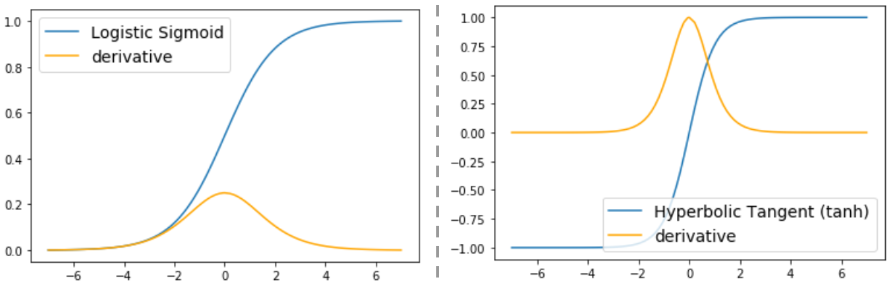
\includegraphics{figure/derivs_sigm_tanh.png}}
      \caption{Sigmoidal activations (Savino \& Tondolo, 2021)}
    \end{figure}
    \item In each case, the function is only sensitive to its inputs in a small neighborhood around $0$.
    \item Furthermore, the derivative is never greater than 1 and is close to zero across much of the domain.
  \end{itemize}
\end{frame}

\begin{vbframe}{Sigmoidal Activation Functions}

\begin{enumerate}
  \item \textbf{Saturating Neurons:}
  \begin{itemize}
    \item We know: $\sigma'\left(z_{in}\right) \to 0$ for $|z_{in}| \to \infty$. 
    \item[$\to$] Neurons with sigmoidal activations "saturate" easily, that is, they stop being responsive when $|z_{in}| \gg 0$. 
  \end{itemize}

  \framebreak 

  \item \textbf{Vanishing Gradients: } Consider the vector of error signals $\bm{\delta}^{(i)}$ in layer $i$ 

    $$
      \bm{\delta}^{(i)} = \Wmat^{(i + 1)} \bm{\delta}^{(i + 1)} \odot \sigma'\left(\bm{z}_{in}^{(i)}\right), i \in\{ 1, ..., O\}. 
    $$

    Each $k$-th component of the vector expresses how much the loss $L$ changes when the input to the $k$-th neuron $z_{k, in}^{(i)}$ changes. 
    \begin{itemize}
      \item We know: $\sigma'(z)< 1$ for all $z \in \mathbb{R}$. 
      \item[$\to$] In each step of the recursive formula above, the value will be multiplied by a value smaller than one
      \begin{eqnarray*}
        \bm{\delta}^{(1)} &=& \Wmat^{(2)} \bm{\delta}^{(2)} \odot \sigma'\left(z_{in}^{(i)}\right) \\
        &=& \Wmat^{(2)} \left(\Wmat^{(3)} \bm{\delta}^{(3)} \odot \sigma'\left(z_{in}^{(i)}\right)\right) \odot \sigma'\left(z_{in}^{(i)}\right) \\
        &=& ...
      \end{eqnarray*}
      \item When this occurs, earlier layers train \emph{very} slowly (or not at all).
    \end{itemize}
\end{enumerate}

\end{vbframe}


\begin{frame} {Rectified Linear Units (ReLU)}
  \begin{itemize}
    \item The ReLU activation solves the vanishing gradient problem.
    \begin{figure}
      \centering
        \scalebox{0.62}{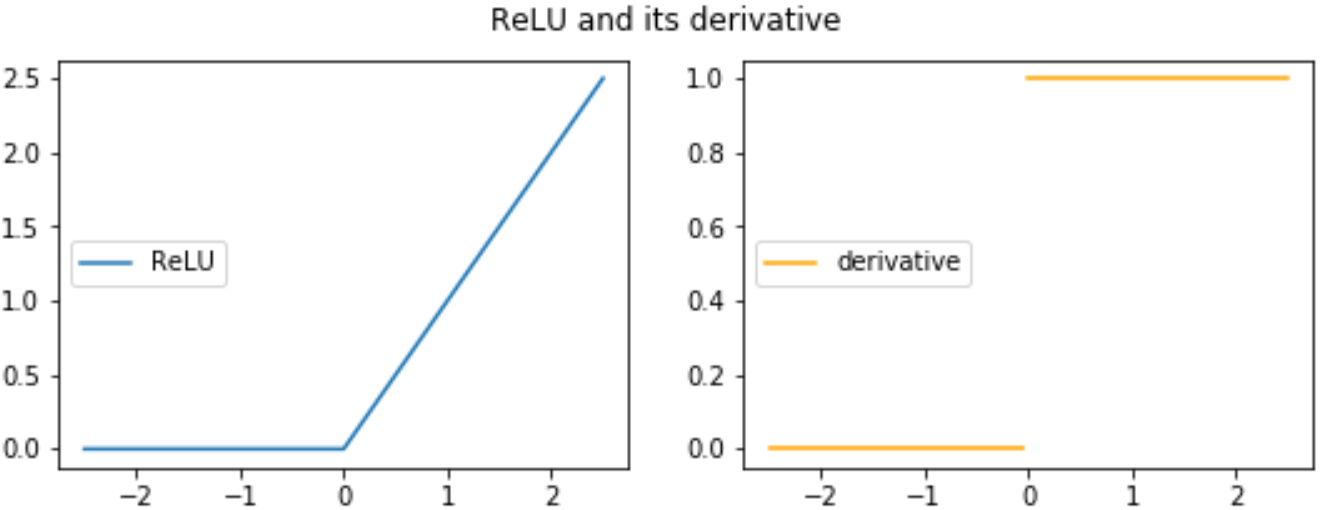
\includegraphics{figure/relu_deriv.png}}
        \caption{ReLU activation (Savino \& Tondolo, 2021)}
    \end{figure}
    \item In regions where the activation is positive, the derivative is $1$. 
    \item Derivatives do not vanish along paths containing "active" neurons.
    \item Note that the ReLU is not differentiable at 0 (Software implementations usually simply return $0$).
  \end{itemize}
\end{frame}

\begin{frame} {Rectified Linear Units (ReLU)}
  \begin{itemize}
    \item ReLU units can significantly speed up training compared to units with saturating activations.
    \begin{figure}
    \centering
      \scalebox{0.48}{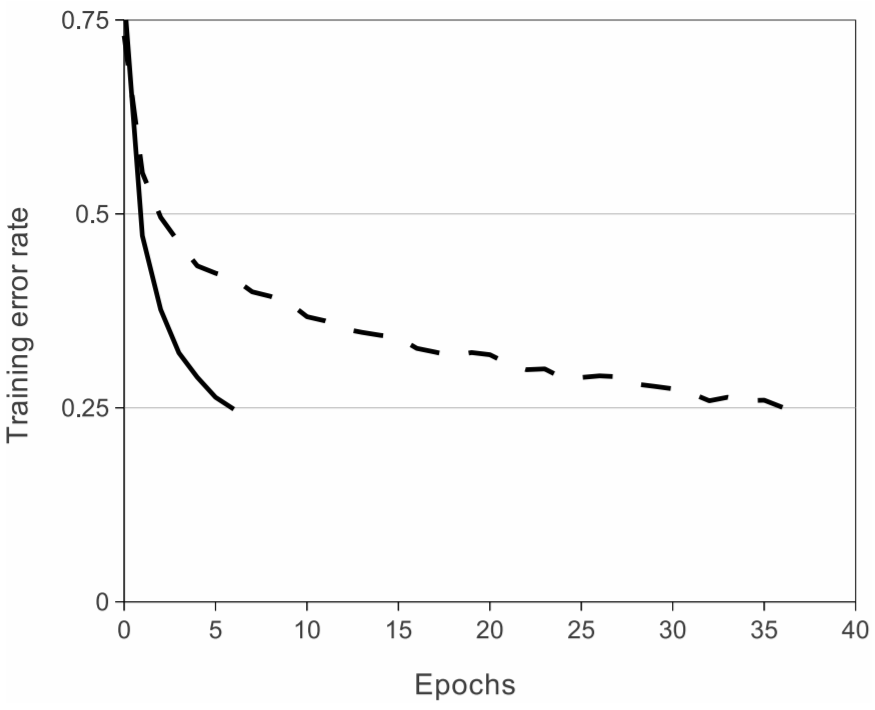
\includegraphics{figure/relu_vs_tanh.png}}
      \caption{\footnotesize A four-layer convolutional neural network with ReLUs (solid line) reaches a 25\% 
training error rate on the CIFAR-10 dataset six times faster than an equivalent network with tanh neurons (dashed line) (Krizhevsky et al., 2012). }
    \end{figure}
  \end{itemize}
\end{frame}

\begin{frame} {Rectified Linear Units (ReLU)}
  \begin{itemize}
  \item A downside of ReLU units is that when the input to the activation is negative, the derivative is zero (the "dying ReLU problem").
    \begin{figure}
      \centering
        \scalebox{0.75}{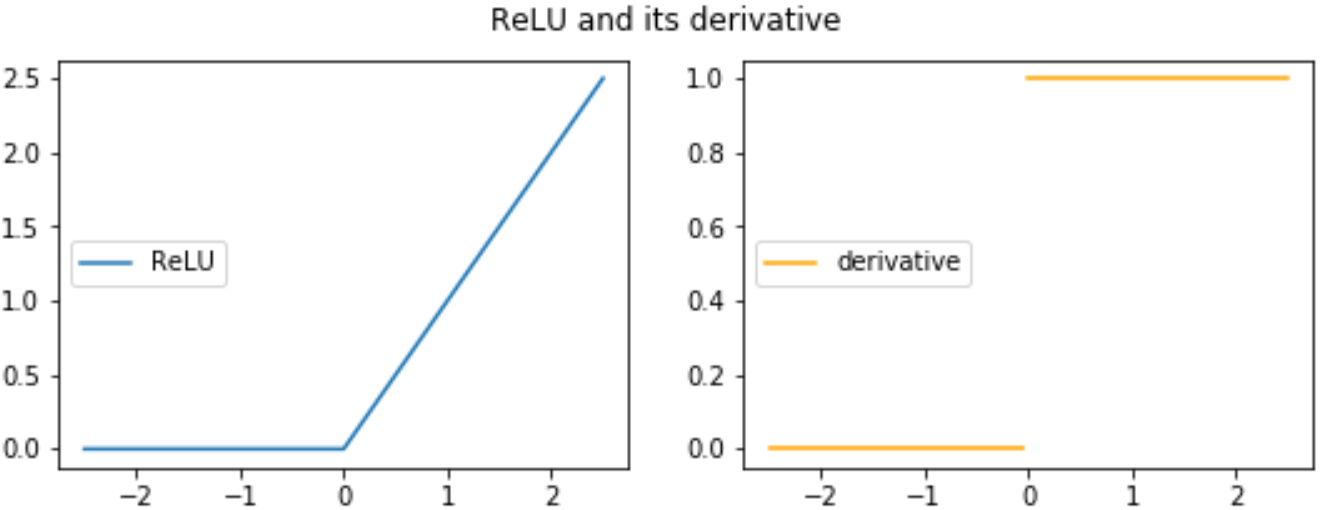
\includegraphics{figure/relu_deriv.png}}
        \caption{ReLU activation (Savino \& Tondolo, 2021)}
    \end{figure}
    \item When a ReLU unit "dies" (i.e.\ its activation is 0 for all datapoints), it kills the gradient flowing during backpropogation.
    \item Such units are never updated during training.
   
  \end{itemize}
\end{frame}

\begin{frame} {Generalizations of ReLU}
  \begin{itemize}
    \item There exist several generalizations of the ReLU activation that have non-zero derivatives throughout their domains.
    \item \emph{Leaky ReLU}: 
    $$  LReLU(v) = \begin{cases} 
          v & v \geq 0 \\
          \alpha v & v < 0 
       \end{cases} $$
    \begin{figure}
      \centering
        \scalebox{0.35}{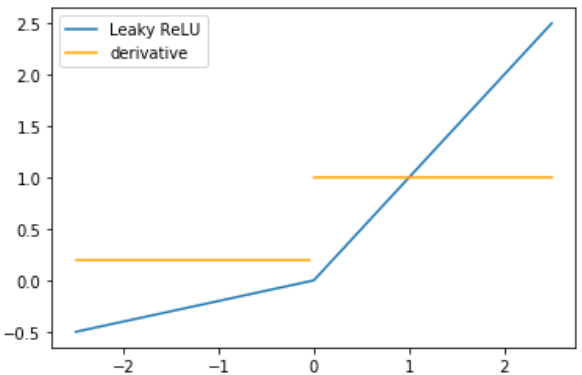
\includegraphics{figure/leakyrelu_deriv.png}}
        \caption{Leaky ReLU (Savino \& Tondolo, 2021)}
    \end{figure}
    \item Unlike the ReLU, when the input to the Leaky ReLU activation is negative, the derivative is $\alpha$ which is a small positive value.
  \end{itemize}
\end{frame}

\begin{frame} {Generalizations of ReLU}
  \begin{itemize}
    \item A variant of the Leaky ReLU is the \emph{Parametric ReLU (PReLU)} which learns the $\alpha$ from the data through backpropagation.

    \item \emph{Exponential Linear Unit (ELU)}:
    
    $$ ELU(v) = \begin{cases} 
          v & v \geq 0 \\
          \alpha (e^v - 1) & v < 0 
       \end{cases} $$

    \item \emph{Scaled Exponential Linear Unit (SELU)}:
    
    $$ SELU(v) = \lambda \begin{cases} 
          v & v \geq 0 \\
          \alpha (e^v - 1) & v < 0 
       \end{cases} $$
  
  {\scriptsize Note: In ELU and SELU, $\alpha$ and $\lambda$ are hyperparameters that are set before training.}
  \item These generalizations may perform as well as or better than the ReLU on some tasks. 
  \end{itemize}

\end{frame}

\begin{frame} {Generalizations of ReLU}
  \lz
  \lz
  \begin{figure}
    \centering
      \scalebox{1}{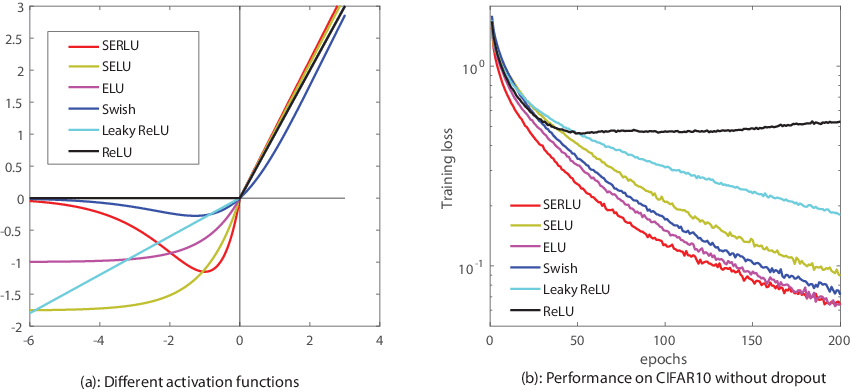
\includegraphics{figure/actfun_comparison.png}}
      \caption{Visualization of different generalisations of ReLU (Zhang et al., 2018)}
      \end{figure}
\end{frame}

% \begin{frame} {Hidden activations}
%   \begin{itemize}
%     \item In general, the design of activation functions is heuristically motivated.
%     \item Choice of hidden units doesn't make many guiding principles.
%     \item Difficult to predict a priori which ones
%     \item Aside from the ones we've seen, it is possible for many other functions to have comparable performance.
%     \item For example, 
%   \end{itemize}
% \end{frame}

\section{Output activations}

\begin{frame} {Output Activations}
  \begin{itemize}
    \item As we have seen previously, the role of the output activation is to get the final score on the same scale as the target.
    \item The output activations and the loss functions used to train neural networks can be viewed through the lens of maximum likelihood estimation (MLE).
    \item In general, the function $f(\xv~|~\thetav)$ represented by the neural network defines the conditional $p(y~|~\xv,\thetav)$ in a supervised learning task.
    \item Maximizing the likelihood is then equivalent to minimizing $- \log p(y~|~\xv,\thetav)$.
    \item An output unit with the identity function as the activation can be used to represent the mean of a Gaussian distribution.
    \item For such a unit, training with mean-squared error is equivalent to maximizing the log-likelihood (ignoring issues with non-convexity).
  \end{itemize}
\end{frame}

\begin{vbframe}{Excursus: Maximum Likelihood Estimation}
  \begin{itemize}
    \item Given i.i.d. training data $(\xv^{(i)}, \yi)_{i \in \nset}$ and a model defining $p(y \mid \xv, \thetav)$, the \textbf{likelihood} is how probable the observed labels are under the model:
    $$L(\thetav) = \prod_{i=1}^n p(\yi \mid \xv^{(i)}, \thetav)$$
    \item \textbf{Maximum likelihood estimation (MLE)} picks the parameters that make the observed data most probable: $\hat{\thetav} = \argmax_{\thetav} L(\thetav)$.
  \end{itemize}
\framebreak

  \begin{itemize}
    \item In practice we use the \textbf{log-likelihood}: $\log$ turns the product into a numerically stable sum, and since $\log$ is monotonic, the maximizer is unchanged:
    $$\log L(\thetav) = \sum_{i=1}^n \log p(\yi \mid \xv^{(i)}, \thetav)$$
    \item Since we usually \textit{minimize} losses, we equivalently minimize the \textbf{negative} log-likelihood: $\hat{\thetav} = \argmin_{\thetav} \left(-\sum_{i=1}^n \log p(\yi \mid \xv^{(i)}, \thetav)\right)$.
    \item This is the bridge used throughout: pick an output activation that defines a distribution, and the matching loss falls out as its negative log-likelihood.
  \end{itemize}
\end{vbframe}


\begin{frame} {Output Activations}
  \small
  \begin{itemize}
    \setlength{\itemsep}{2pt}
    \item Similarly, sigmoid and softmax units can output the parameter(s) of a Bernoulli distribution and Categorical distribution, respectively.
    \item It is straightforward to show that when the label is one-hot encoded, training with the cross-entropy loss is equivalent to maximizing log-likelihood. \href{https://www.quora.com/What-are-the-differences-between-maximum-likelihood-and-cross-entropy-as-a-loss-function}{\beamergotobutton{Click here}}
    \item Because these activations can saturate, an important advantage of maximizing log-likelihood is that the $\log$ undoes some of the exponentiation in the activation functions which is desirable when optimizing with gradient-based methods.
    \item For example, in the case of softmax, the loss is:
    $$ L(y, \fx) = - f_{in,k} + \log {\sum_{k'=1}^g\exp(f_{in,k'})}$$ where $k$ is the correct class. The first term, $- f_{in,k}$, does not saturate which means training can progress steadily even if the contribution of $f_{in,k}$ to the second term is negligible.
  \end{itemize}
\end{frame}

\begin{frame} {Output Activations}
  \begin{itemize}
    \item A neural network can even be used to output the parameters of more complex distributions.
    \item A Mixture Density Network, for example, outputs the parameters of a Gaussian Mixture Model:
$$p(y | \xv)=\sum_{c=1}^{m} \phi^{(c)} (\xv) ~ \mathcal{N}\left(y ; \boldsymbol{\mu}^{(c)}(\xv), \boldsymbol{\Sigma}^{(c)}(\xv)\right)$$
          where $m$ the number of components in the mixture.
    \item In such a network, the output units are divided into groups.
    \item One group of output neurons with softmax activation represents the weights ($\phi^{(c)}$) of the mixture.
    \item Another group with the identity activation represents the means ($\boldsymbol{\mu}^{(c)}$) and yet another group with a non-negative activation function (such as ReLU or the exponential function) can represent the variances of the (typically) diagonal covariance matrices $\boldsymbol{\Sigma}^{(c)}$.
  \end{itemize}
\end{frame}

\begin{frame} {Output Activations}
  \begin{figure}
    \centering
      \scalebox{1}{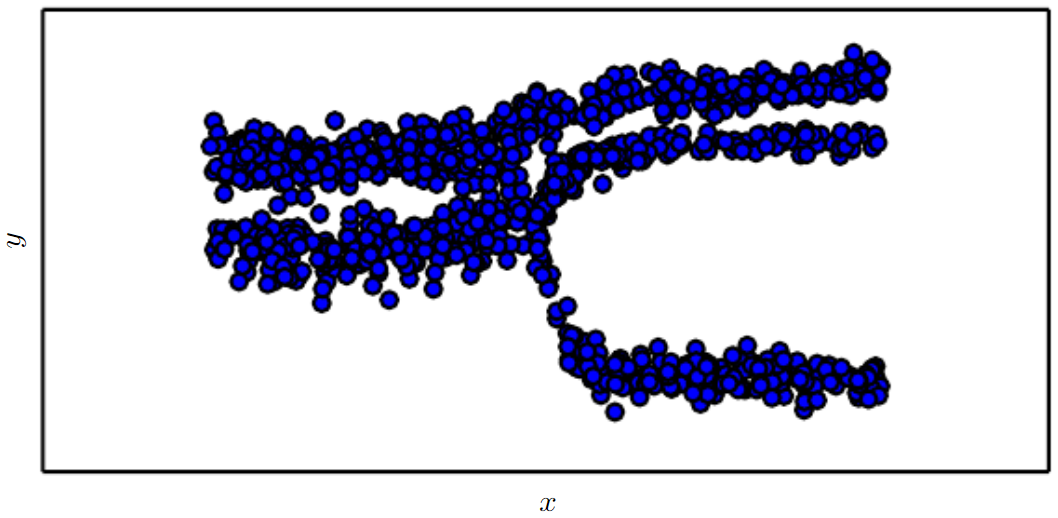
\includegraphics{figure/mdn.png}}
      \caption{\footnotesize Samples drawn from a Mixture Density Network. The input $\xv$ is sampled from a uniform distribution and $y$ is sampled from $p(y~|~\xv,\thetav)$ (Goodfellow et al., 2016).}
  \end{figure}
\end{frame}

%%%%%%%%%%%%%%%%%%%%%%%%%%%%%%%%%%%%%%%%%%%%%%%%%%%%%%%%%%%%%%%%%%
%%%%%%%%%%%%%%%%%%          REFERENCES          %%%%%%%%%%%%%%%%%%
%%%%%%%%%%%%%%%%%%%%%%%%%%%%%%%%%%%%%%%%%%%%%%%%%%%%%%%%%%%%%%%%%%
\begin{vbframe}
\frametitle{References}
\footnotesize{
\begin{thebibliography}{99}
%%%%%%%%%%%%%%%%%%%%%%%%%%%%%%%%%%
\bibitem[(Savino \& Tondolo, 2021)]{act1}Savino, P., \& Tondolo, F. (2021). Automated classification of civil structure defects based on convolutional neural network. \textit{Frontiers of Structural and Civil Engineering, 15}(2), 305–317. \url{https://doi.org/10.1007/s11709-021-0725-9}


\bibitem[Ian Goodfellow et al., 2016]{act2} 
Goodfellow, I., Bengio, Y., \& Courville, A. (2016). \textit{Deep Learning}. MIT Press.

%%%%%%%%%%%%%%%%%%%%%%%%%%%%%%%%%%
\bibitem[(Krizhevsky et al., 2012)]{act3} 
Krizhevsky, A., Sutskever, I., \& Hinton, G. E. (2012). ImageNet Classification with Deep Convolutional Neural Networks. In F. Pereira, C. J. Burges, L. Bottou, \& K. Q. Weinberger (Eds.), \textit{Advances in Neural Information Processing Systems} (Vol. 25). Curran Associates, Inc. \url{https://proceedings.neurips.cc/paper_files/paper/2012/file/c399862d3b9d6b76c8436e924a68c45b-Paper.pdf}

%%%%%%%%%%%%%%%%%%%%%%%%%%%%%%%%%%
\bibitem[(Zhang et al., 2018)]{act4}
Zhang, G., \& Li, H. (2018). \textit{Effectiveness of Scaled Exponentially-Regularized Linear Units (SERLUs)}.

\end{thebibliography}
}
\end{vbframe}
%%%%%%%%%%%%%%%%%%%%%%%%%%%%%%%%%%%%%%%%%%%%%%%%%%%%%%%%%%%%%%%%%%
%%%%%%%%%%%%%%%%%%%%%%%%%%%%%%%%%%%%%%%%%%%%%%%%%%%%%%%%%%%%%%%%%%


\section{Loss Functions}

\begin{vbframe}{What Is a Loss Function?}
\begin{itemize}
\item A \textbf{loss function} $\Lxy$ quantifies point-wise how we measure
errors in predictions for a single $\xv$: $$L: \mathcal{Y} \times \R^g \to \R.$$
\item The \textbf{theoretical risk} of a candidate model $f$ is the expected
loss: $$\mathcal{R}(f) := \mathbb{E}_{xy}[\Lxy] = \int \Lxy ~ d\mathbb{P}_{xy},$$
the average error we incur when using $f$ on data from $\mathbb{P}_{xy}$. Since
$\mathbb{P}_{xy}$ is unknown, we cannot compute this directly.
\item Instead, given $n$ i.i.d. training observations, we approximate it by
the \textbf{empirical risk}: $$\riske = \frac{1}{n}\sumin \Lxyit.$$
\item \textbf{Empirical risk minimization (ERM)} finds $\hat{\thetav} =
\argmin_{\thetav} \riske$, usually via numerical optimization.
\end{itemize}
\end{vbframe}

\begin{vbframe}{Regression: L2 and L1 Loss}
\begin{itemize}
\item For regression, we typically use the L2 (squared-error) loss:
$$\Lxy = \frac{1}{2}(y - \fx)^2$$
\item For a single neuron, this loss is convex; the global optimum can be found
with gradient descent, or in this special case analytically via the normal
equations.
\item An alternative is the L1 (absolute-error) loss:
$$\Lxy = |y - \fx|$$
\item L2 loss is minimized (in expectation) by the conditional mean of $y$
given $\xv$; L1 loss is minimized by the conditional median. L1 is therefore
more robust to outliers, but its loss surface is non-differentiable at $0$.
\end{itemize}
\framebreak

\begin{figure}
\centering
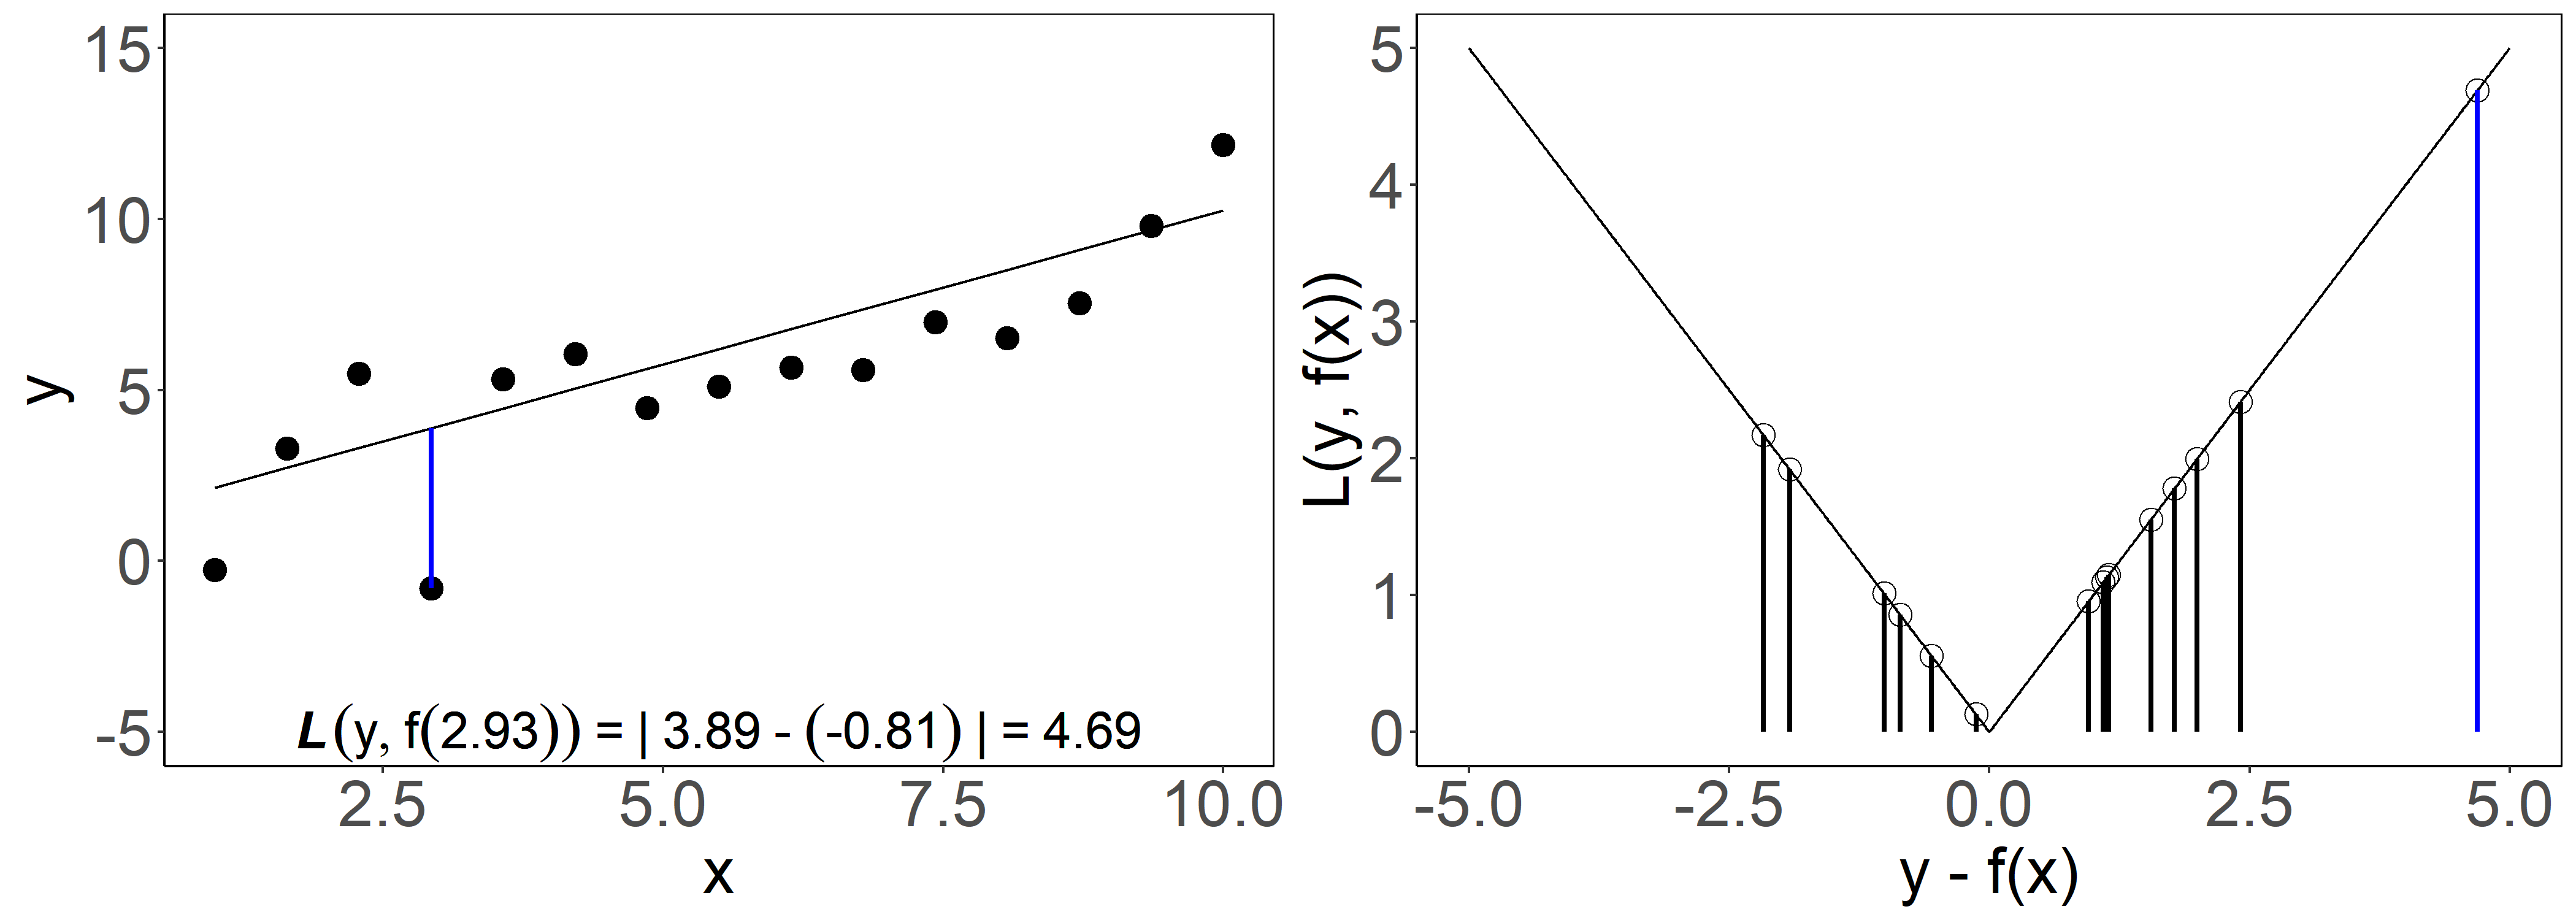
\includegraphics[width=11cm]{figure/i2ml-l1-loss.png}
\caption{\footnotesize L1 loss: per-observation loss (left) and the loss curve $L(y,f(\xv))$ against the residual $y - f(\xv)$ (right). Source: SLDS LMU, I2ML.}
\end{figure}
\framebreak

\begin{figure}
\centering
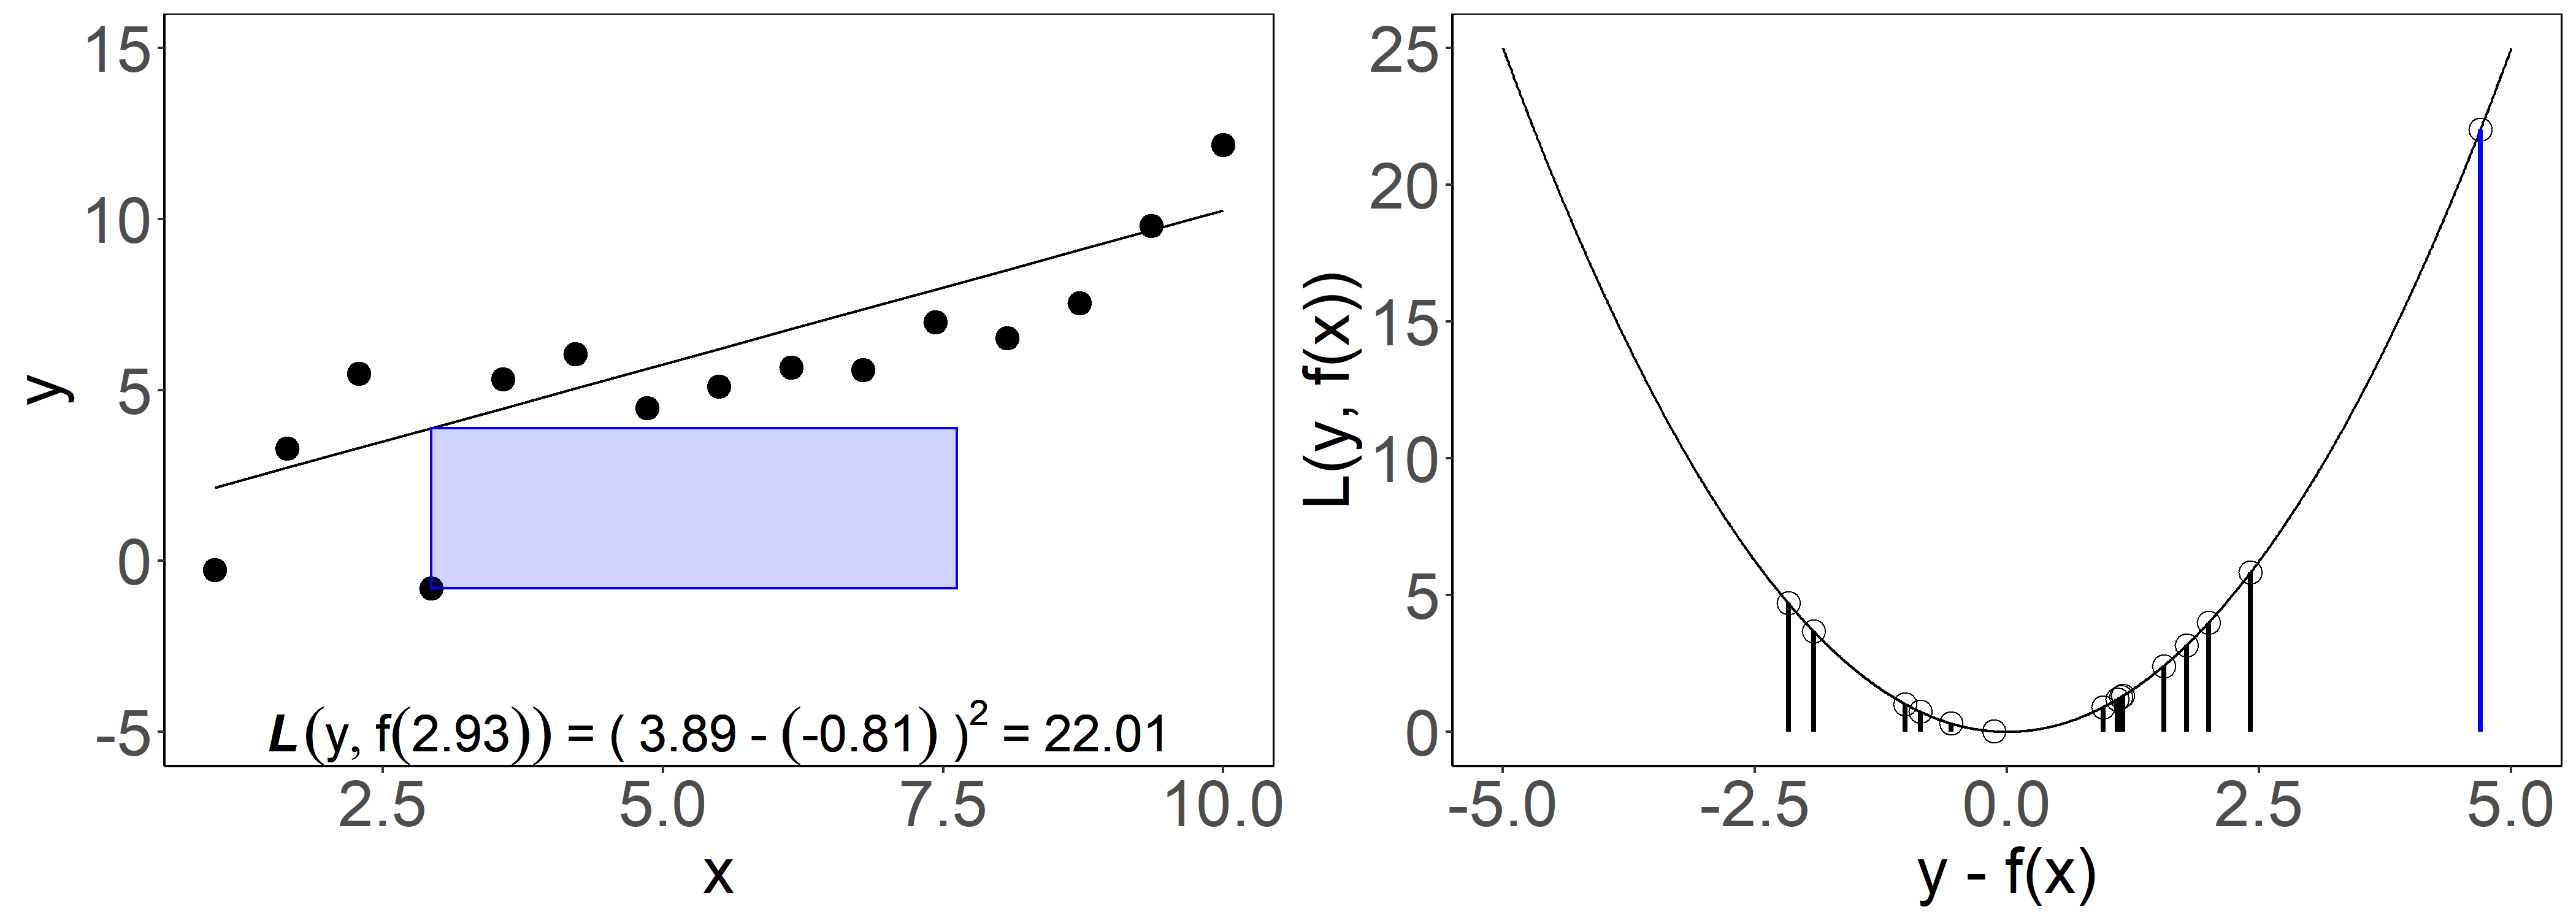
\includegraphics[width=11cm]{figure/i2ml-l2-loss.png}
\caption{\footnotesize L2 loss: per-observation loss (left) and the loss curve $L(y,f(\xv))$ against the residual $y - f(\xv)$ (right). Source: SLDS LMU, I2ML.}
\end{figure}
\end{vbframe}

\begin{vbframe}{Binary Classification: Cross-Entropy Loss}
\begin{itemize}
\item For binary classification, we typically apply the cross-entropy loss
(also known as Bernoulli loss):
$$\Lxy = -(y \log \fx + (1 - y) \log(1 - \fx))$$
\item A single neuron with logistic sigmoid activation trained with the
Bernoulli loss yields the same result as logistic regression trained until
convergence.
\end{itemize}
\end{vbframe}

\begin{vbframe}{Multi-Class Classification: Softmax Loss}
\begin{itemize}
\item For $g$-class classification, the softmax loss is
$$L(y, \fx) = - \sum_{k = 1}^g [y = k] \log \left( \frac{\exp(f_{in,k})}{\sum_{k'=1}^g\exp(f_{in,k'})}\right)$$
\item This is equivalent to the cross-entropy loss when the label vector
$\bm{y}$ is one-hot coded.
\item A numerically more stable, equivalent form is
$$ L(y, \fx) = - f_{in,k} + \log {\sum_{k'=1}^g\exp(f_{in,k'})}$$
where $k$ is the correct class: the first term does not saturate, so training
progresses steadily even when $f_{in,k}$'s contribution to the second term is
negligible.
\end{itemize}
\end{vbframe}

\begin{vbframe}{Losses as Maximum Likelihood}
\begin{itemize}
\item Output activations and loss functions can be viewed through the lens of
maximum likelihood estimation (MLE): the network's output defines a
conditional distribution $p(y~|~\xv,\thetav)$, and maximizing the likelihood
is equivalent to minimizing $-\log p(y~|~\xv,\thetav)$.
\item An identity output activation trained with mean-squared error is
equivalent to maximizing the log-likelihood under a Gaussian distribution.
\item Sigmoid/softmax output activations trained with cross-entropy loss are
equivalent to maximizing the log-likelihood under a Bernoulli/Categorical
distribution, respectively.
\end{itemize}
\end{vbframe}

%%%%%%%%%%%%%%%%%%%%%%%%%%%%%%%%%%%%%%%%%%%%%%%%%%%%%%%%%%%%%%%%%%
%%%%%%%%%%%%%%%%%%          REFERENCES          %%%%%%%%%%%%%%%%%%
%%%%%%%%%%%%%%%%%%%%%%%%%%%%%%%%%%%%%%%%%%%%%%%%%%%%%%%%%%%%%%%%%%
\begin{vbframe}
\frametitle{References}
\footnotesize{
\begin{thebibliography}{99}
\bibitem[(SLDS LMU)]{loss1} SLDS LMU. \textit{Introduction to Machine Learning
(I2ML)}, chapter \enquote{Losses \& Risk Minimization}.
\url{https://slds-lmu.github.io/i2ml/chapters/01_ml_basics/01-06-riskminimization/}
\end{thebibliography}
}
\end{vbframe}

\section{Basic Regularization}
%%%%%%%%%%%%%%%%%%%%%%%%%%%%%%%%%%%%%%%%%%%%%%%%%%%%%%%%%%%%%%%%%%

\begin{frame} {Regularization}
\begin{itemize}
\item Any technique that is designed to reduce the test error possibly at the expense of increased training error can be considered a form of regularization.
\item Regularization is important in DL because NNs can have extremely high capacity (millions of parameters) and are thus prone to overfitting.
\end{itemize}
\end{frame}
%%%%%%%%%%%%%%%%%%%%%%%%%%%%%%%%%%%%%%%%%%%%%%%%%%%%%%%%%%%%%%%%%%

\begin{vbframe}{Revision: Regularized Risk Minimization}
\begin{itemize}
\item The goal of regularized risk minimization is to penalize the complexity of the model to minimize the chances of overfitting.
\item By adding a parameter norm penalty term \(J(\thetav)\) to the empirical risk $\risket$ we obtain a regularized cost function:
$$\riskrt = \risket + \lambda \text{\(J(\thetav)\)}$$
with hyperparamater $\lambda \in [0, \infty)$, that weights the penalty term, relative to the unconstrained objective function $\risket$.
\item Therefore, instead of pure \textbf{empirical risk minimization}, we add a penalty
for complex (read: large) parameters \(\thetav\).
\item Declaring $\lambda = 0$ obviously results in no penalization.
\item We can choose between different parameter norm penalties \(J(\thetav)\).
\item In general, we do not penalize the bias.
\end{itemize}
\end{vbframe}
%%%%%%%%%%%%%%%%%%%%%%%%%%%%%%%%%%%%%%%%%%%%%%%%%%%%%%%%%%%%%%%%%%

\begin{vbframe}{L2-regularization / Weight decay}
Let us optimize the L2-regularized risk of a model $\fxt$
\[\min_{\thetav} \riskrt = \min_{\thetav} \risket + \frac{\lambda}{2} \|\thetav\|^2_2\]
by gradient descent. The gradient is
\[\nabla \riskrt = \nabla \risket + \lambda \thetav.\]
We iteratively update $\thetav$ by step size \(\alpha\) times the
negative gradient
\[\thetav^{[\text{t+1}]} = \thetav^{[\text{t}]} - \alpha \left(\nabla \risket + \lambda \thetav^{[\text{t}]}\right) =
\thetav^{[\text{t}]} (1 - \alpha \lambda) - \alpha \nabla \risket\]
$\to$ The term \(\lambda \thetav^{[t]}\) causes the parameter
(\textbf{weight}) to \textbf{decay} in proportion to its size (which gives rise to the name). 
\end{vbframe}

%%%%%%%%%%%%%%%%%%%%%%%%%%%%%%%%%%%%%%%%%%%%%%%%%%%%%%%%%%%%%%%%%%

\begin{frame}{Equivalence to Constrained Optimization}
Norm penalties can be interpreted as imposing a constraint on the weights. One can show that 
 $$\argmin_{\theta} \risket + \lambda \text{\(J(\thetav)\)}$$
 is equvilalent to
 \begin{align*}
 & \argmin_{\thetav}  \risket \\
  &\text{subject to \;\;\;}  J(\thetav) \leq k
 \end{align*}
  for some value $k$ that depends on $\lambda$ and $\risket$ (Goodfellow et al., 2016)
\end{frame}
%%%%%%%%%%%%%%%%%%%%%%%%%%%%%%%%%%%%%%%%%%%%%%%%%%%%%%%%%%%%%%%%%%

\begin{vbframe}{Example: Weight decay}
\begin{minipage}{0.45\textwidth}
\begin{itemize}
\item We fit the huge neural network on the right side on a smaller fraction of MNIST (5000 train and 1000 test observations)
\item Weight decay: $\lambda \in (10^{-2}, 10^{-3}, 10^{-4}, 10^{-5}, 0)$
\end{itemize}
\end{minipage}
\begin{minipage}{0.45\textwidth}
\begin{figure}
\centering
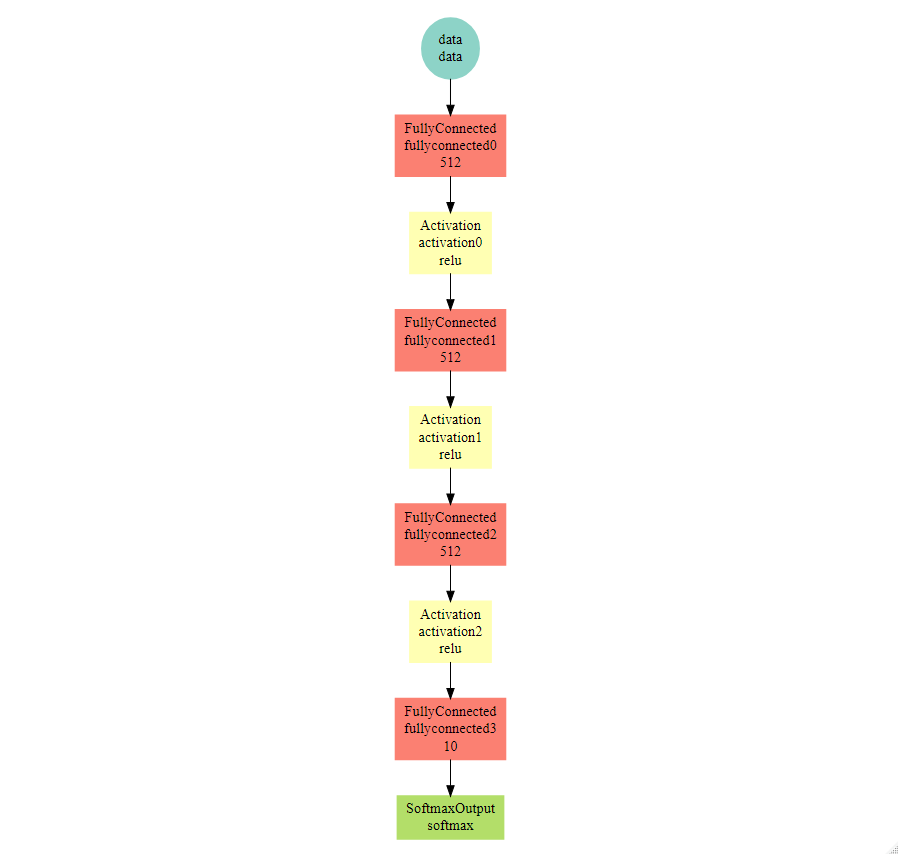
\includegraphics[width= 8.7cm, height=7.7cm]{figure/mxnet_graph_decay.png}
\end{figure}
\end{minipage}
\framebreak
%%%%%%%%%%%%%%%%%%%%%%%%%%%%%%%%%%%%%%%%%%%%%%%%%%%%%%%%%%%%%%%%%%

\begin{figure}
\centering
\scalebox{1}{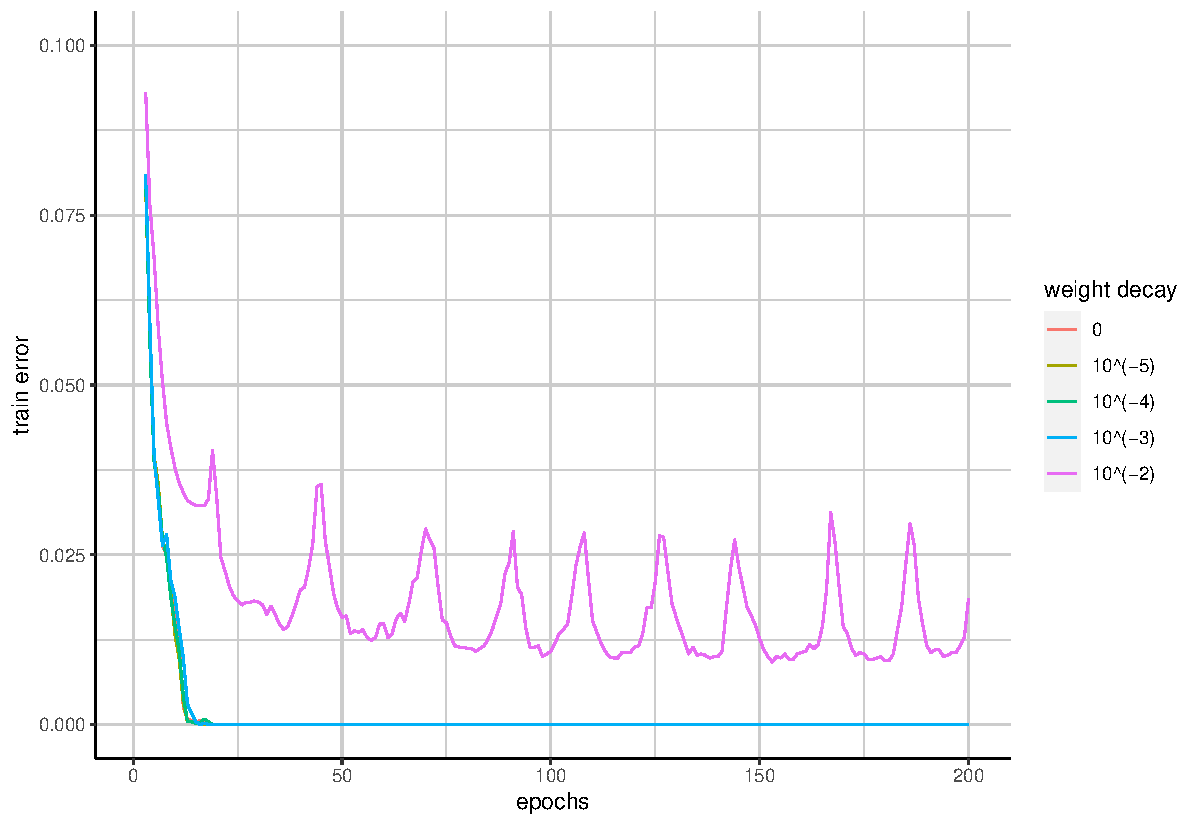
\includegraphics{figure/weight_decay1.pdf}}
\\
A high weight decay of $10^{-2}$ leads to a high error on the training data.
\end{figure}

\framebreak
%%%%%%%%%%%%%%%%%%%%%%%%%%%%%%%%%%%%%%%%%%%%%%%%%%%%%%%%%%%%%%%%%%

\begin{figure}
\centering
\scalebox{1}{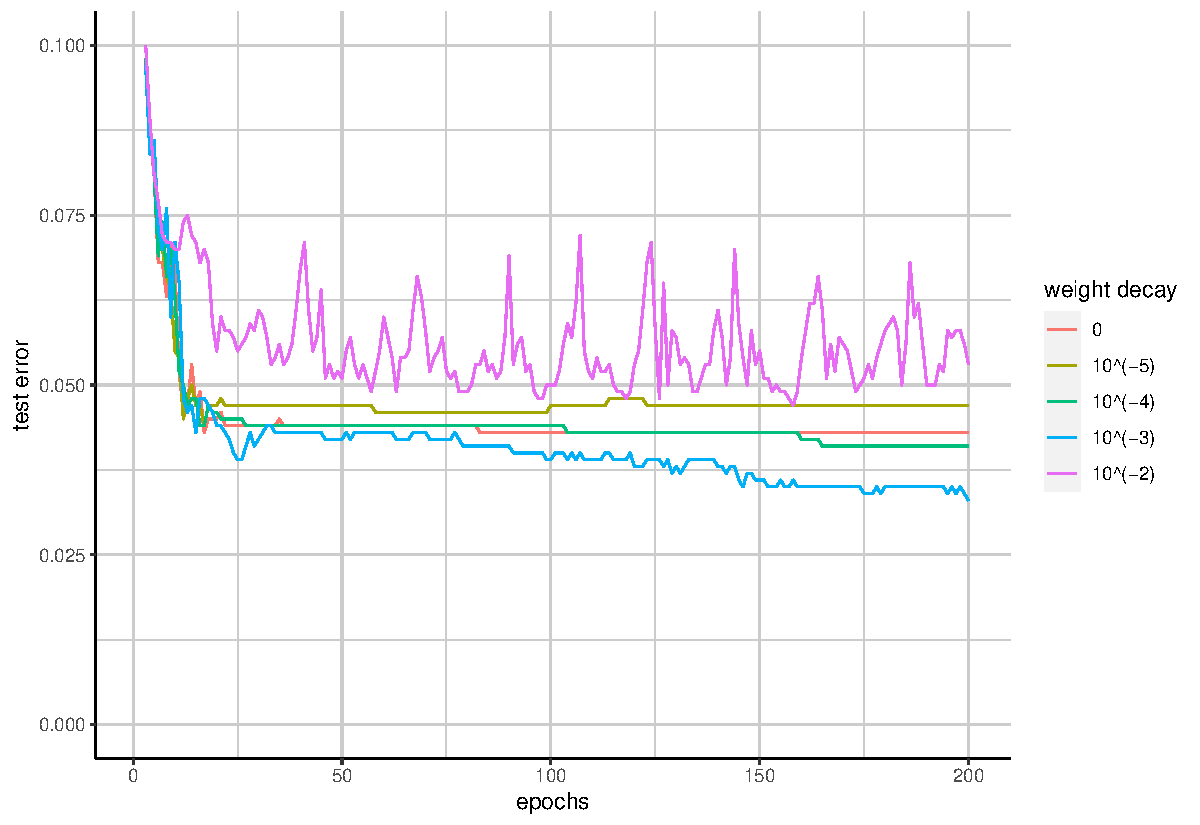
\includegraphics{figure/weight_decay2.pdf}}
\\
Second strongest weight decay leads to the best result on the test data.
\end{figure}
\end{vbframe}
  
%%%%%%%%%%%%%%%%%%%%%%%%%%%%%%%%%%%%%%%%%%%%%%%%%%%%%%%%%%%%%%%%%%
\begin{frame}{Tensorflow Playground}
\begin{figure}
\centering
\scalebox{0.8}{
\includegraphics{figure/tensorflow_playground.png}}
  \caption{\url{https://playground.tensorflow.org/}, (Carter)}
  \end{figure}
\end{frame}

\begin{frame}{Tensorflow Playground - Exercise}
  \begin{figure}
    \centering
      \scalebox{0.8}{
\includegraphics{figure/tensorflow_exercise.png}}
    \caption{\url{https://developers.google.com/machine-learning/crash-course/regularization-for-simplicity/playground-exercise-examining-l2-regularization} (Google)}
  \end{figure}
\end{frame}

%%%%%%%%%%%%%%%%%%%%%%%%%%%%%%%%%%%%%%%%%%%%%%%%%%%%%%%%%%%%%%%%%%
%%%%%%%%%%%%%%%%%%%%%%%%%%%%%%%%%%%%%%%%%%%%%%%%%%%%%%%%%%%%%%%%%%
%%%%%%%%%%%%%%%%%%          REFERENCES          %%%%%%%%%%%%%%%%%%
%%%%%%%%%%%%%%%%%%%%%%%%%%%%%%%%%%%%%%%%%%%%%%%%%%%%%%%%%%%%%%%%%%
\begin{vbframe}
\frametitle{References}
\footnotesize{
\begin{thebibliography}{99}
%%%%%%%%%%%%%%%%%%%%%%%%%%%%%%%%%%
\bibitem[(Goodfellow, 2016)]{reg1} 
Goodfellow, I., Bengio, Y., \& Courville, A. (2016). \textit{Deep Learning}. MIT Press. 
%%%%%%%%%%%%%%%%%%%%%%%%%%%%%%%%%%
\bibitem[(MathWorks)]{reg2} 
MathWorks. (n.d.). \textit{Regularization}. MATLAB \& Simulink. \url{https://de.mathworks.com/discovery/regularization.html}
%%%%%%%%%%%%%%%%%%%%%%%%%%%%%%%%%%
\bibitem[(Carter)]{reg3} 
Carter, D. S. and S. (n.d.). \textit{Tensorflow - Neural Network Playground. A Neural Network Playground}. \url{https://playground.tensorflow.org} 
%%%%%%%%%%%%%%%%%%%%%%%%%%%%%%%%%%
\bibitem[(Google)]{reg4} Google. (n.d.). \textit{Regularization for Simplicity: Playground Exercise (L2 Regularization)}. Google. \url{https://developers.google.com/machine-learning/crash-course/regularization-for-simplicity/playground-exercise-examining-l2-regularization?hl=de} 
\end{thebibliography}
}
\end{vbframe}
%%%%%%%%%%%%%%%%%%%%%%%%%%%%%%%%%%%%%%%%%%%%%%%%%%%%%%%%%%%%%%%%%%
%%%%%%%%%%%%%%%%%%%%%%%%%%%%%%%%%%%%%%%%%%%%%%%%%%%%%%%%%%%%%%%%%%


\section{Early Stopping}

\begin{vbframe}{Early Stopping}
  
  \begin{itemize}
    \item When training with an iterative optimizer such as SGD, it is commonly the case that, after a certain number of iterations, generalization error begins to increase even though training error continues to decrease.     
    \item \textbf{Early stopping} refers to stopping the algorithm early before the generalization error increases.
  \end{itemize}
  \begin{figure}
    \centering
      \scalebox{0.5}{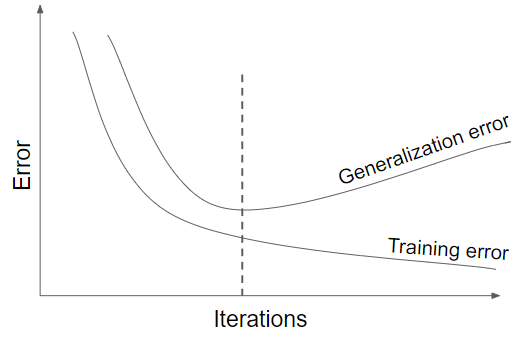
\includegraphics{figure/earlystop.png}}
      \caption{After a certain number of iterations, the algorithm begins to overfit.}
  \end{figure}
\end{vbframe}


%%%%%%%%%%%%%%%%%%%%%%%%%%%%%%%%%%%%%%%%%%%%%%%%%%%%%%%%%%%%%%%%%%
%%%%%%%%%%%%%%%%%%%%%%%%%%%%%%%%%%%%%%%%%%%%%%%%%%%%%%%%%%%%%%%%%%
\section{Ensemble Methods}
\begin{vbframe}{Recap: Ensemble Methods}

\begin{itemize}
\item Idea: Train \textbf{several models} separately, and \textbf{average their prediction} (i.e.~perform \textbf{model averaging}).
%$$\frac{1}{k} \sum_{i=1}^k f_k(x|\theta)$$
\item Intuition: This improves performance on test set, since different models will not make the same errors.
\item Ensembles can be constructed in different ways, e.g.:
\begin{itemize}
\item by combining completely different kind of models (using different learning algorithms and loss functions).
\item by \textbf{bagging}: train the same model on $k$ datasets, constructed by sampling $n$ samples from original dataset.
\end{itemize}
\item Since training a neural network repeatedly on the same dataset results in different solutions (why?) it can even make sense to combine those.
\end{itemize}

\framebreak 

\begin{figure}
    \centering
      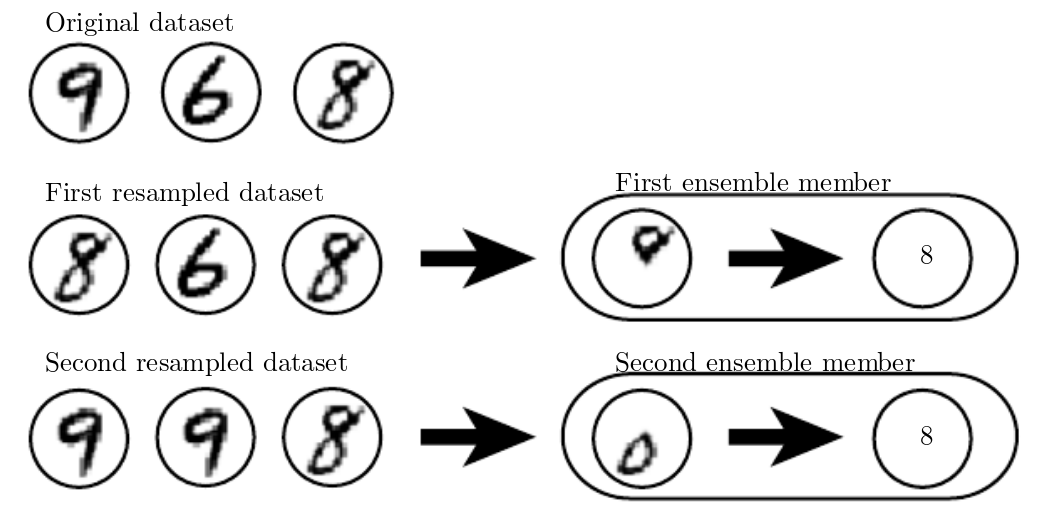
\includegraphics[width=11cm]{figure/bagging.png}
      \caption{A cartoon description of bagging (Goodfellow et al., 2016)}
  \end{figure}

\end{vbframe}
%%%%%%%%%%%%%%%%%%%%%%%%%%%%%%%%%%%%%%%%%%%%%%%%%%%%%%%%%%%%%%%%%%
%%%%%%%%%%%%%%%%%%%%%%%%%%%%%%%%%%%%%%%%%%%%%%%%%%%%%%%%%%%%%%%%%%
\section{Dropout}

\begin{vbframe}{Dropout}
  \begin{itemize}
    \item %Dropout is a regularization technique for
    Idea: reduce overfitting in neural networks by preventing complex co-adaptations of neurons.
    \item Dropout can be seen as a form of "model averaging".
    \item Method: during training, random subsets of the neurons are removed from the network (they are "dropped out").This is done by artificially setting the activations of those neurons to zero.
    \item Whether a given unit/neuron is dropped out or not is completely independent of the other units.
    \item If the network has $N$ (input/hidden) units, applying dropout to these units can result in $2^N$ possible 'subnetworks'.
    \item Because these subnetworks are derived from the same 'parent' network, many of the weights are shared.
  \end{itemize}
\framebreak
  \begin{figure}
    \centering
      \scalebox{0.8}{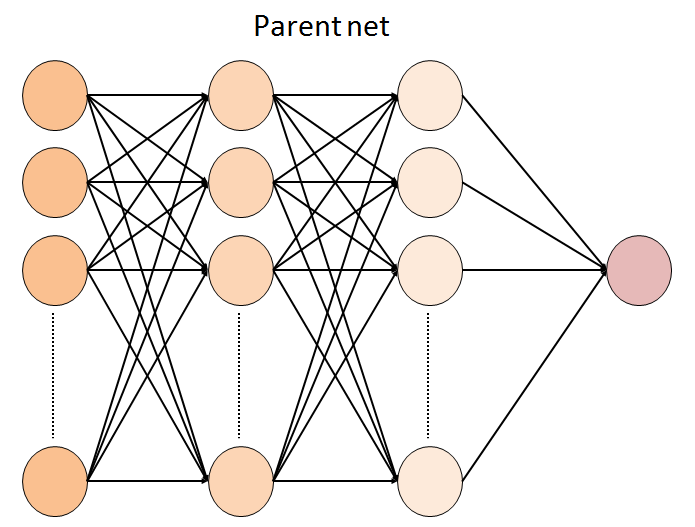
\includegraphics{figure/dropout.png}}
  \end{figure}
\framebreak
  \begin{figure}
    \centering
      \scalebox{0.8}{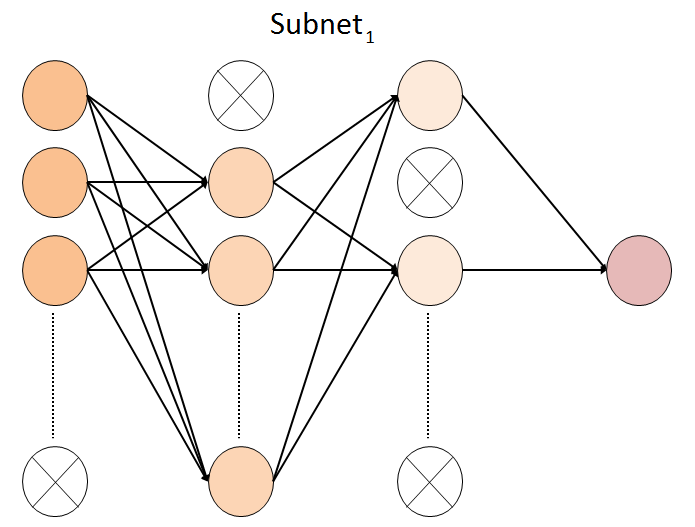
\includegraphics[width=10cm]{figure/subnet1.png}}
  \end{figure}
  In each iteration, for each training example (in the forward pass), a different (random) subset of neurons are dropped out.
\framebreak
  \begin{figure}
    \centering
      \scalebox{0.8}{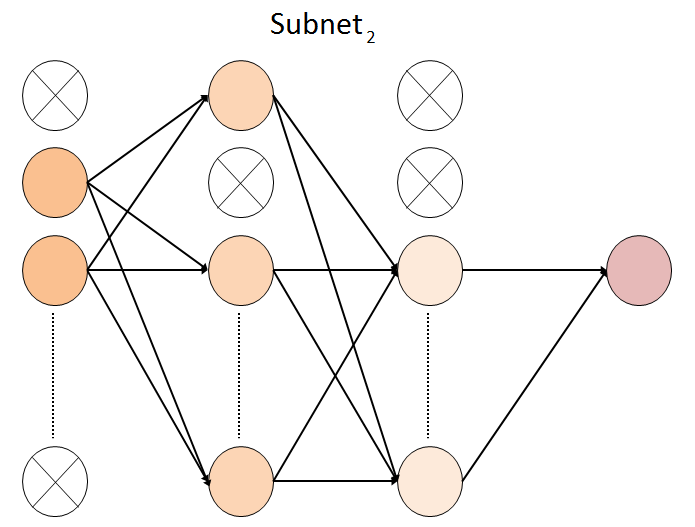
\includegraphics[width=10cm]{figure/subnet2.png}}
  \end{figure}
  In each iteration, for each training example (in the forward pass), a different (random) subset of neurons are dropped out.
\framebreak
  \begin{figure}
    \centering
      \scalebox{0.8}{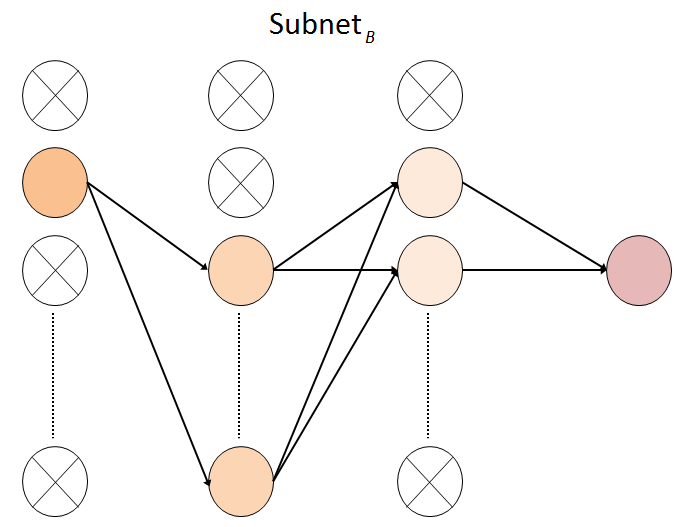
\includegraphics[width=10cm]{figure/subnet3.png}}
  \end{figure}
  In each iteration, for each training example (in the forward pass), a different (random) subset of neurons are dropped out.
\end{vbframe}


\begin{vbframe}{Dropout: Algorithm}
  \begin{itemize}
    \item To train with dropout a minibatch-based learning algorithm such as stochastic gradient descent is used.  
    \item For each training case in a minibatch, we randomly sample a binary vector/mask $\mu$ with one entry for each input or hidden unit in the network. The entries of $\mu$ are sampled independently from each other. 
    \item The probability $p$ of sampling a mask value of 0 (dropout) for one unit is a hyperparameter known as the 'dropout rate'. 
    \item A typical value for the dropout rate is $0.2$ for input units and $0.5$ for hidden units. 
    \item Each unit in the network is multiplied by the corresponding mask value resulting in a $subnet_{\mu}$. 
    \item Forward propagation, backpropagation, and the learning update are run as usual.
  \framebreak
  \begin{algorithm}[H]
  \footnotesize
  \caption{Training a (parent) neural network with dropout rate $p$}
    \begin{algorithmic}[1]
      \State Define parent network and initialize weights
      \For{each minibatch: }
        \For{each training sample: }
        \State Draw mask $\mu$ using $p$
        \State Compute forward pass for $subnet_{\mu}$
%        \State Compute the gradient of the loss for $network_{\mu}$
        \EndFor
        \State \parbox[t]{\dimexpr\linewidth-\algorithmicindent}{Update the weights of the (parent) network by performing a gradient descent step with weight decay}
      \EndFor
    \end{algorithmic}
  \end{algorithm}
    \item The derivatives wrt. each parameter are averaged over the training cases in each mini-batch. Any training case which does not use a parameter contributes a gradient of zero for that parameter.
      \end{itemize}
\end{vbframe}

\begin{vbframe}{Dropout: Weight scaling}
  \begin{itemize}
    \item The weights of the network will be larger than normal because of dropout. Therefore, to obtain a prediction at test time the weights must be first scaled by the chosen dropout rate.
    \item This means that if a unit (neuron) is retrained with probability $p$ during training, the weight at test time of that unit is multiplied by $p$.
  \begin{figure}
      \centering
    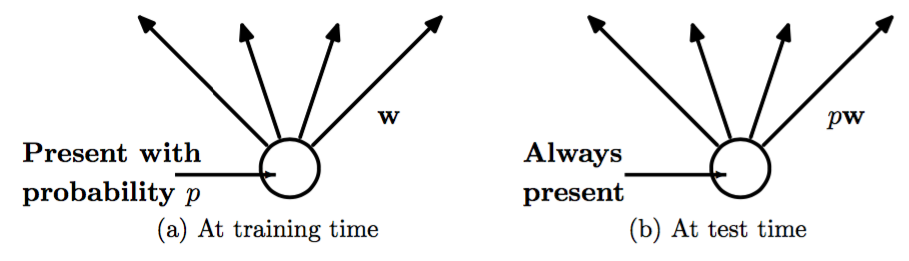
\includegraphics[width=7cm]{figure/dropout_neuron.png}
    \caption{Training vs. Testing (Srivastava et. al., 2014)}
  \end{figure}
  \item Weight scaling ensures that the expected total input to a neuron/unit at test time is roughly the same as the expected total input to that unit at train time, even though many of the units at train time were missing on average
  \item Rescaling of the weights can also be performed at training time instead, after each weight update at the end of the mini-batch. This is sometimes called 'inverse dropout'. Keras and PyTorch deep learning libraries implement dropout in this way.
 % \item Weight scaling ensures that for any hidden unit the \textbf{expected} output (under the distribution used to drop units at training time) is the same as the \textbf{actual} output at test time. 
  \end{itemize}
\end{vbframe}

%%%%%%%%%%%%%%%%%%%%%%%%%%%%%%%%%%%%%%%%%%%%%%%%%%%%%%%%%
\begin{vbframe}{Dropout: Example}
\begin{minipage}{0.5\textwidth}
  \begin{itemize}
    \item To demonstrate how dropout can easily improve generalization we compute neural networks with the structure showed on the right.
    \item Each neural network we fit has different dropout probabilities, a tuple where one probability is for the input layer and one is for the hidden layers. We consider the tuples $(0;0) , (0.2;0.2) \text{ and } (0.6;0.5)$.
  \end{itemize}
  \end{minipage}
  \begin{minipage}{0.45\textwidth}
  \begin{figure}
    \centering
    \vspace{-0.5cm}
      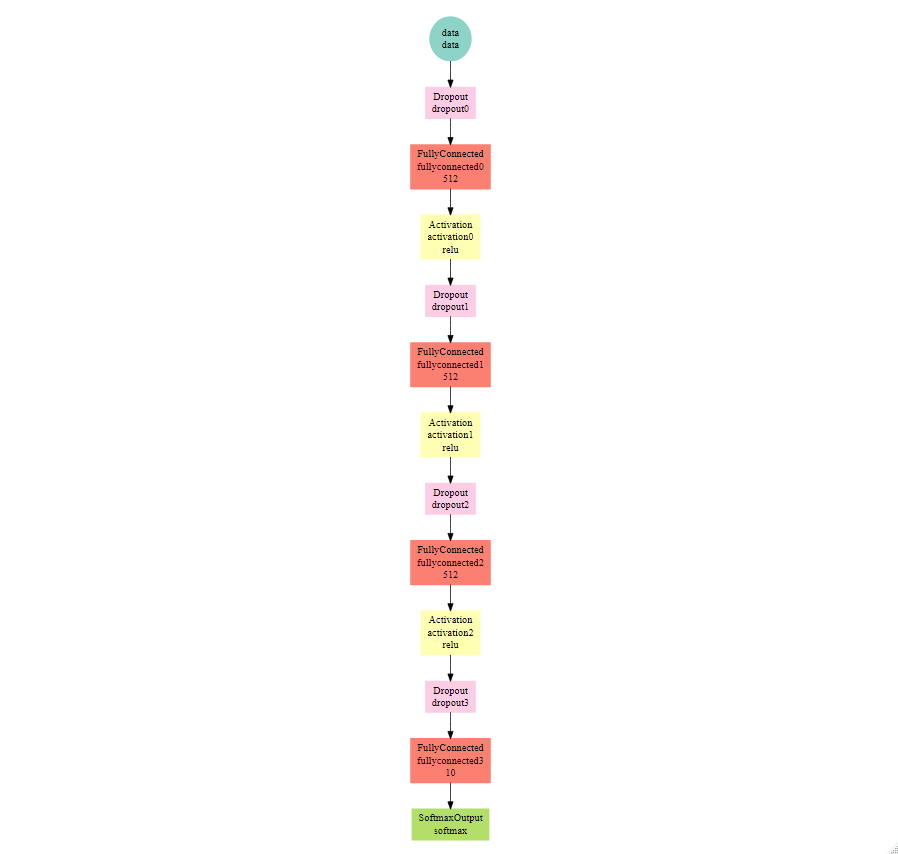
\includegraphics[width=9cm]{figure/mxnet_graph_dropout.png}
  \end{figure}
  \end{minipage}
\framebreak
%
%\begin{knitrout}\scriptsize
%\definecolor{shadecolor}{rgb}{0.969, 0.969, 0.969}\color{fgcolor}
%
%{\centering \includegraphics[width=0.95\textwidth]{figure/unnamed-chunk-3-1} 
%
%}
%
%
%\end{knitrout}
%Higher dropout rates lead to higher training error. 
%\framebreak

\begin{knitrout}\scriptsize
\definecolor{shadecolor}{rgb}{0.969, 0.969, 0.969}\color{fgcolor}

{\centering 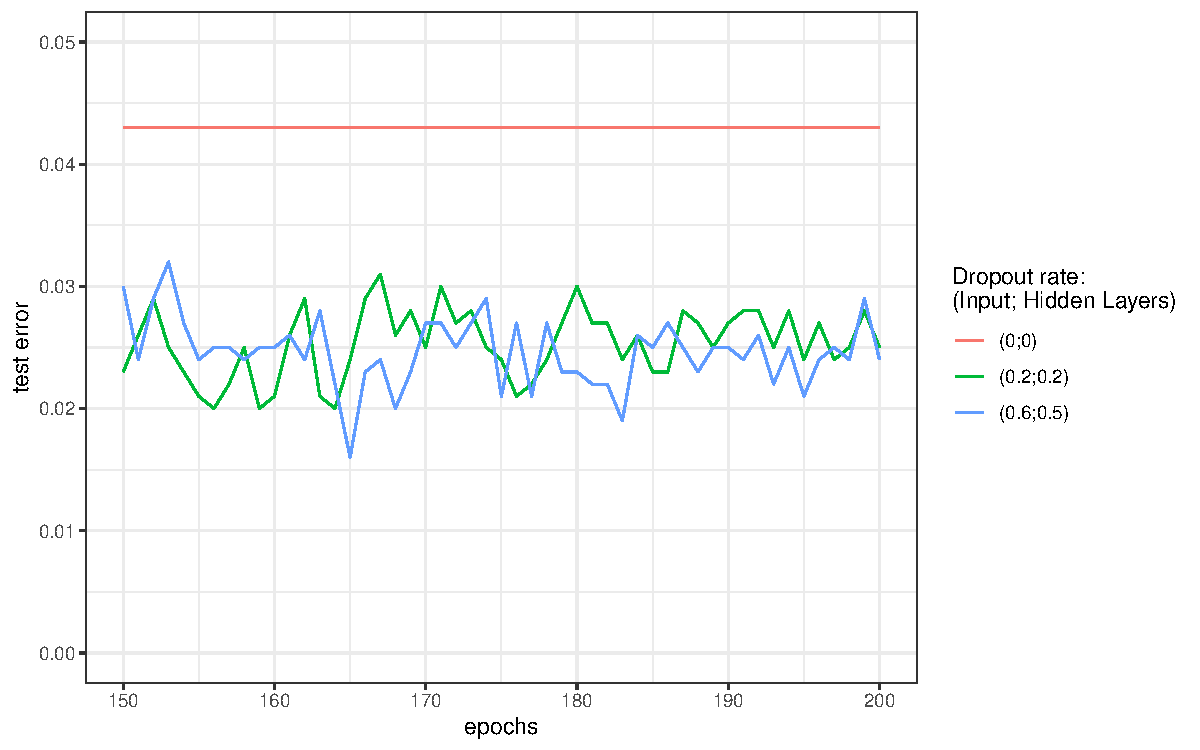
\includegraphics[width=0.95\textwidth]{figure/unnamed-chunk-4-1} 

}


\end{knitrout}
Dropout rate of 0 (no dropouts) leads to higher test error than dropping some units out. 
\end{vbframe}
%%%%%%%%%%%%%%%%%%%%%%%%%%%%%%%%%%%%%%%%%%%%%%%%%%%%%%%%%%%%%%%%%%
%%%%%%%%%%%%%%%%%%%%%%%%%%%%%%%%%%%%%%%%%%%%%%%%%%%%%%%%%%%%%%%%%%
\begin{vbframe}{Dropout, weight decay or both?}

\begin{knitrout}\scriptsize
\definecolor{shadecolor}{rgb}{0.969, 0.969, 0.969}\color{fgcolor}

{\centering 
\includegraphics[width=0.95\textwidth]{figure/unnamed-chunk-5-1} 

}


\end{knitrout}
Here, dropout leads to a smaller test error than using no regularization or solely weight decay. 
\end{vbframe}
%%%%%%%%%%%%%%%%%%%%%%%%%%%%%%%%%%%%%%%%%%%%%%%%%%%%%%%%%%%%%%%%%%
%%%%%%%%%%%%%%%%%%%%%%%%%%%%%%%%%%%%%%%%%%%%%%%%%%%%%%%%%%%%%%%%%%

\section{Dataset Augmentation}
\begin{vbframe}{Dataset Augmentation}
  \begin{itemize}
    \item Problem: low generalization because high ratio of $$\frac{\text{complexity of the model}}{\text{\#train data}}$$
    \item Idea: artificially increase the train data.
      \begin{itemize}
        \item Limited data supply $\rightarrow$ create \enquote{fake data}! 
      \end{itemize}
    \item Increase variation in inputs \textbf{without} changing the labels.
    \item Application:
      \begin{itemize}
        \item Image and Object recognition (rotation, scaling, pixel translation, flipping, noise injection, vignetting, color casting, lens distortion, injection of random negatives)
        \item Speech recognition (speed augmentation, vocal tract perturbation)
      \end{itemize}
  \end{itemize}
\framebreak
  \begin{figure}
    \centering
      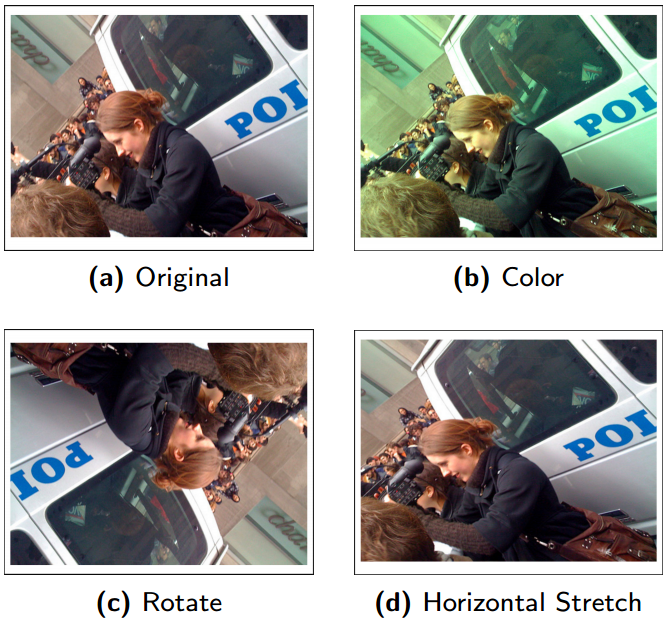
\includegraphics[width=7cm]{figure/data_augmentation_1.png}
      \caption{Example for data set augmentation (Wu et al., 2015)}
  \end{figure}
\framebreak
  \begin{figure}
    \centering
      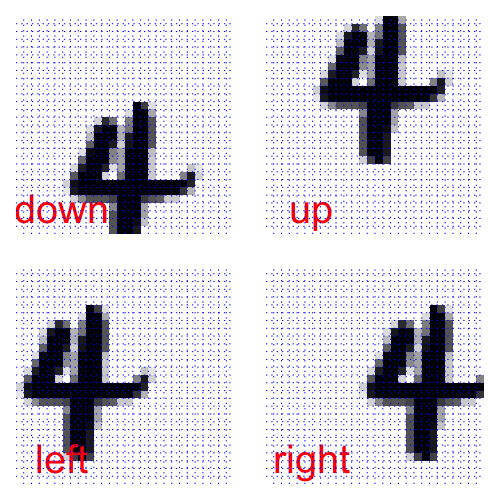
\includegraphics[width=6cm]{figure/data_augmentation_2.png}
      \caption{Example for data set augmentation (Wu et al., 2015)}
  \end{figure}
  $\Rightarrow$ careful when rotating digits (6 will become 9 and vice versa)!
\end{vbframe}
%%%%%%%%%%%%%%%%%%%%%%%%%%%%%%%%%%%%%%%%%%%%%%%%%%%%%%%%%%%%%%%%%%
%%%%%%%%%%%%%%%%%%%%%%%%%%%%%%%%%%%%%%%%%%%%%%%%%%%%%%%%%%%%%%%%%%
%\section{Noise Robustness}
%\begin{vbframe}{Artificial Noise}
%Idea: Intentionally inject noise to the model, e.g.~inject noise 
%  \begin{itemize} 
%    \item  \textbf{to the input} to make the model more robust to small variations.
%  %  \item This method may force the model to \enquote{grow} weights in regions of flat minima. Thus, the noisy model may not find perfect minima but its approximations lie in a flatter surrounding.
%   (Bishop (1995) shows that for some models this has the same effect as parameter norm penalization.)
%   \item \textbf{to the weights}, which can interpreted as stochastic implementation of Bayesian inference and pushes the model to flat minima in parameter space. 
%    \item \textbf{to the outputs}  to account for possible errors in the labeling process. E.g.,~for \textbf{label smoothing} one replaces the label $1$ of a correct class by $1-\epsilon$ and the label $0$ of the $g$ remaining by $\frac{\epsilon}{g-1}$.
%    %In practice, it is common to apply noise to the outputs. This strategy is termed label smoothing as it incorporates a small noise term on the labels of the classification outputs. The intuition is to account for possible errors in the labeling process.
%  \end{itemize}
%\end{vbframe}
%


%%%%%%%%%%%%%%%%%%%%%%%%%%%%%%%%%%%%%%%%%%%%%%%%%%%%%%%%%%%%%%%%%%

%%%%%%%%%%%%%%%%%%%%%%%%%%%%%%%%%%%%%%%%%%%%%%%%%%%%%%%%%%%%%%%%%%
%%%%%%%%%%%%%%%%%%          REFERENCES          %%%%%%%%%%%%%%%%%%
%%%%%%%%%%%%%%%%%%%%%%%%%%%%%%%%%%%%%%%%%%%%%%%%%%%%%%%%%%%%%%%%%%
\begin{vbframe}
\frametitle{References}
\footnotesize{
\begin{thebibliography}{99}
%%%%%%%%%%%%%%%%%%%%%%%%%%%%%%%%%%
\bibitem[Ian Goodfellow et al., 2016]{dropaug1} Goodfellow, I., Bengio, Y., \& Courville, A. (2016). \textit{Deep Learning}. MIT Press. 
%%%%%%%%%%%%%%%%%%%%%%%%%%%%%%%%%%
\bibitem[Hinton et al., 2012]{dropaug2} Hinton, G. E., Srivastava , N., Krizhevsky , A., Sutskever , I., \& Salakhutdinov, R. R. (2012). Improving neural networks by preventing co-adaptation of feature detectors. 
%%%%%%%%%%%%%%%%%%%%%%%%%%%%%%%%%%
    \bibitem[Srivastava et. al., 2014]{dropaug3} Srivastava, N., Hinton, G., Krizhevsky, A., Sutskever, I., \& Salakhutdinov, R. (2014). Dropout: A Simple Way to Prevent Neural Networks from Overfitting. Journal of Machine Learning Research, 15(56), 1929–1958. \url{http://jmlr.org/papers/v15/srivastava14a.html}
%   %%%%%%%%%%%%%%%%%%%%%%%%%%%%%%%%%%
\bibitem[Wu et al., 2015]{dropaug4} Wu, R., Yan, S., Shan, Y., Dang, Q., \& Sun, G. (2015). Deep Image: Scaling up Image Recognition. 
%   %%%%%%%%%%%%%%%%%%%%%%%%%%%%%%%%%%
%\bibitem[Bishop, Chris M., 1995]{dropaug5} Bishop, Chris M. (1995)
%\newblock Training with Noise is Equivalent to Tikhonov Regularization
%\newblock \emph{\url{https://www.microsoft.com/en-us/research/wp-content/uploads/2016/02/bishop-tikhonov-nc-95.pdf}}


\end{thebibliography}
}
\end{vbframe}
%%%%%%%%%%%%%%%%%%%%%%%%%%%%%%%%%%%%%%%%%%%%%%%%%%%%%%%%%%%%%%%%%%
%%%%%%%%%%%%%%%%%%%%%%%%%%%%%%%%%%%%%%%%%%%%%%%%%%%%%%%%%%%%%%%%%%

\begin{vbframe}{License \& Attribution}
\begin{itemize}
\item Activations and Regularization sections adapted from
\textbf{Introduction to Deep Learning (I2DL)}, Prof.\ Dr.\ Bernd Bischl,
Statistical Learning and Data Science (SLDS), LMU Munich.
\url{https://github.com/slds-lmu/lecture_i2dl} --- licensed
\textbf{CC BY 4.0}: \url{https://creativecommons.org/licenses/by/4.0/}
\item Loss Functions section assembled from \textbf{Introduction to Machine
Learning (I2ML)}, SLDS, LMU Munich. \url{https://github.com/slds-lmu/i2ml}
--- licensed \textbf{MIT}.
\item Content has been merged, reordered, and consolidated from the
original sources into this single session deck; not used verbatim.
\end{itemize}
\end{vbframe}

\endlecture
\end{document}
